\documentclass[12pt]{kupaper}
\usepackage{jtygm}%%%%%%%%%%%%%%%%%Font Warning対策%%%%%
\usepackage[dvipdfmx]{graphicx}
\usepackage{bmpsize}
\usepackage{here}
\usepackage{comment}
\usepackage{amsmath}
\usepackage{booktabs}
\usepackage[dvipdfmx,colorlinks=false]{hyperref}
\usepackage{pxjahyper}
\usepackage{titlesec}
\usepackage{wrapfig}
\usepackage{enumerate}
\usepackage{physics}

\begin{document}

%%% includeはできるだけつかわないでください!!

%論文タイトル
\Title{論文執筆要領}
%論文著者
\Author{橋本 勇輝}
%指導教員
\Professor{馬塲 一晴}
%学籍番号
\StudentNumber{212270040}
%提出日
\Date{6}%2022 卒論用
\Date{6}%2023 修論用

\title{How to write a master's thesis}
\author{Yuki Hashimoto}
\professor{Kazuharu Bamba}
\endate{February}{15}{2023} %2022 卒論用
\endate{February}{2}{2025}  %2023 修論用

%学部の人は次のコメント行の%を外してください.
%\senior
%この\seniorは\Abstractの前であればどこに書いてもかまいません.

\Maketitle

%\setcounter{chapter}{20}
% 目次  (LaTeX の処理を少くする目的で,最後に書いています)
\pagenumbering{roman}
\setcounter{page}{1}
\tableofcontents

\begin{comment} %必要に応じて利用してください.
\clearpage
\listoffigures
\clearpage
\listoftables
\end{comment}

\chapter{序論}
\pagenumbering{arabic} % 絶対必要です.最初の章にのみ記述します.

卒業論文・修士論文は,みなさんのこれまでの研究の成果をまとめて報告し,みなさんがそれぞれの学位に値するかを審査するための重要な論文です.そのためには,これまでの研究成果の内容をよく吟味し,「人に自分の考えを伝える」重要性と難しさに注意し,分かりやすい表現を考え,書いた文章をよく推敲し,さらに,論文として定められた形式をとる必要があります\cite{G_ng_r_2021}.

\begin{equation}
	\qty( \int_0^1 x^2 dx )
\end{equation}

\chapter{メディアおよび必要部数}
\begin{itemize}
	\item 卒業論文:冊子体1部および電子版 (PDFファイル)
	\item 修士論文:冊子体3部\footnote{論文審査委員が4名以上の場合は,その人数分の部数を準備すること.}および電子版 (PDFファイル)
\end{itemize}

\chapter{提出および投稿の締切日時}
\begin{itemize}
	\item 卒業論文:2024年1月20日 (木) 17時
	\item 修士論文:2023年1月31日 (金) 17時
\end{itemize}

\chapter{提出先および投稿先}
提出可能時期については,各年度の執筆概要を参照してください.
\begin{itemize}
	\item 冊子体:指導教員,副指導教員
	\item 電子版:馬塲研究室のGoogleドライブフォルダ \url{https://drive.google.com/drive/folders/18YB1iv1um4TMOjJ7DmGlwVGVjya5adMA?usp=sharing}
\end{itemize}

\chapter{冊子体の体裁}

冊子体は電子版と全く同じ内容の文書を印刷し,製本したものとします.製本には市販の簡易ファイル等を使ってください.製本完成時の全体の体裁を図1に示します.指導教員の指導に従い,表表紙および背表紙には所定の事項を記載し綴じてください.所定の事項は,黒色のペンを用いて手書きするか,プリンタで印字したものを貼付けてください.製本の際には,論文の左側約 13 mmの位置に孔を二つ開けて綴じてください.

\begin{figure}[htbp]
	\centering
	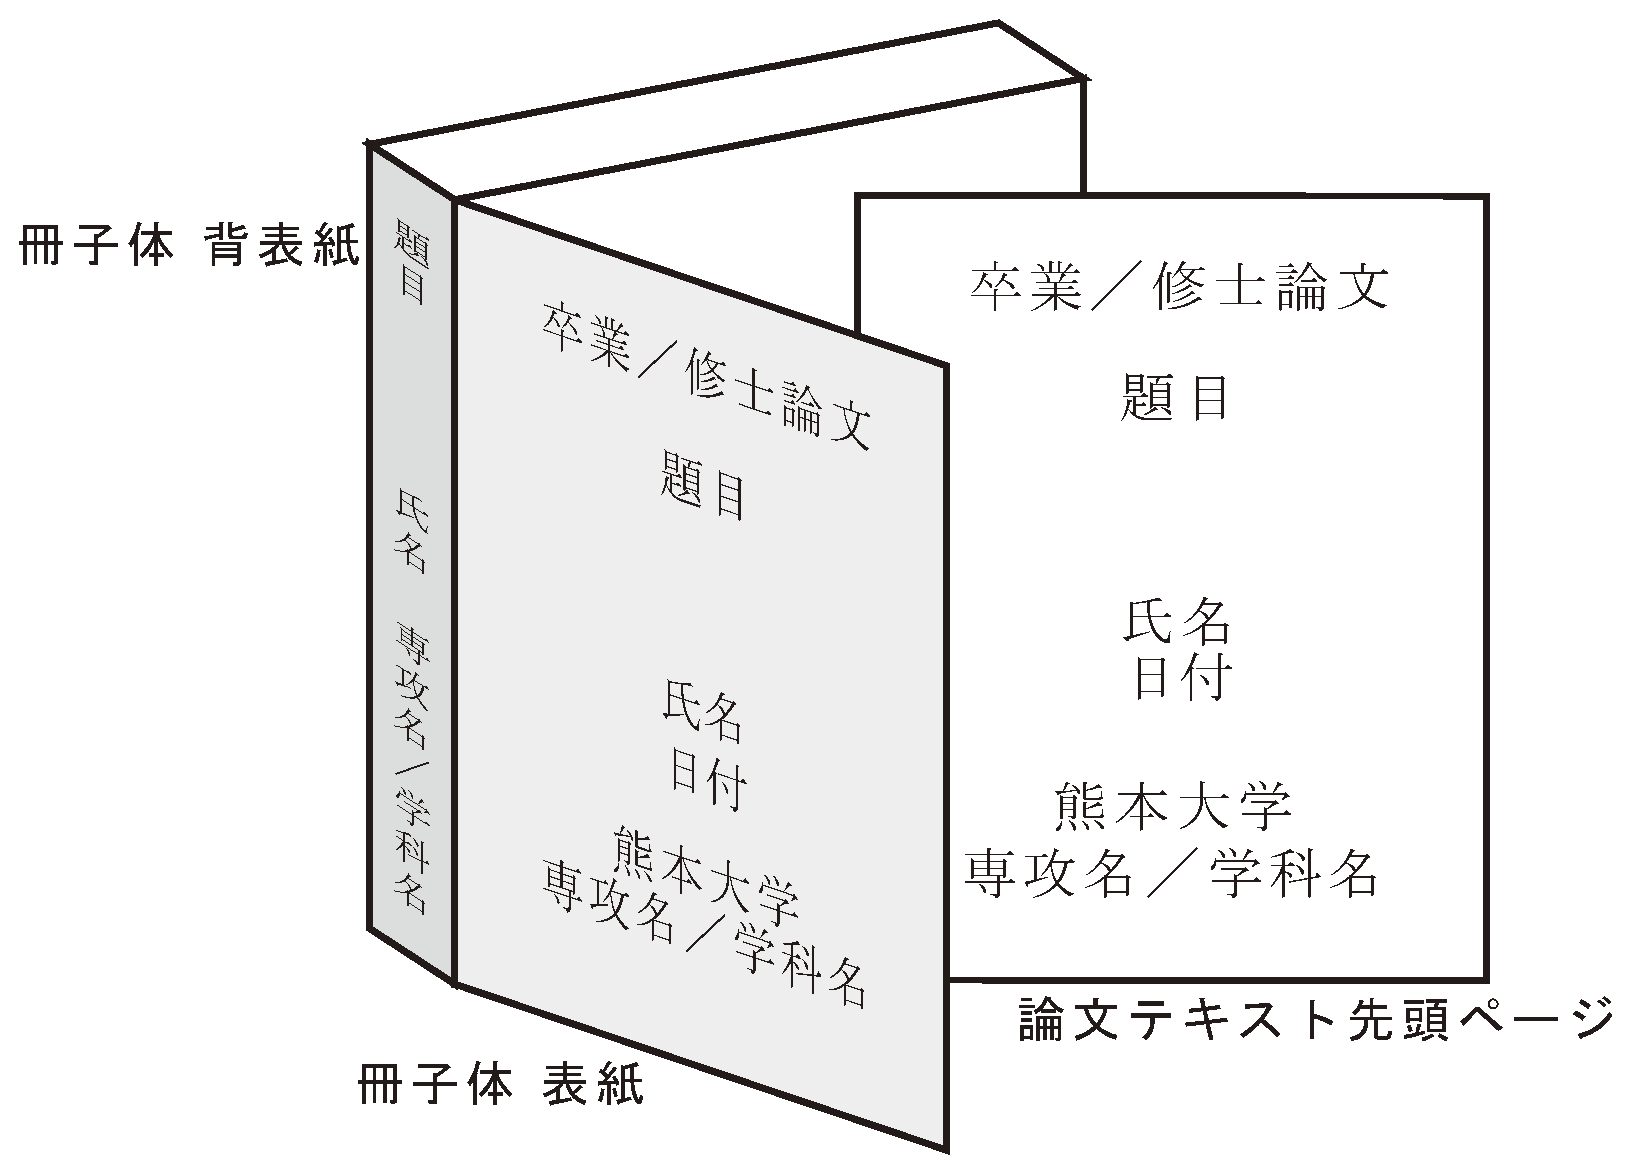
\includegraphics[width=1.0\linewidth,keepaspectratio]{book.eps}
	\caption{冊子体および論文テキストの先頭ページ}
	\label{overview}
\end{figure}

%\vspace*{-3em}
なお,論文テキストの先頭ページには題目・学籍番号・指名・指導教員名・大学名・学科 (コース) 名・提出日を記載してください.これらの印字位置は図\ref{overview}に従って調整してください.


\chapter{論文の構成} \label{論文の構成}
論文は,以下の\ref{a}~\ref{f}の順序で構成してください.



\begin{enumerate}[a.]
	\item 論文テキスト先頭ページ:図\ref{overview}のように記載してください.\label{a}
	\item 目次\label{c}
	\item 本文\label{d}
	\item 謝辞\label{e}
	\item 参考文献\label{f}
\end{enumerate}

\chapter{論文の記述要領}
\begin{enumerate}[a.]
	\item 文書作成ソフトウェア等で作成してください.なお,電子版はPDF形式で投稿してください.
	\item 用紙のサイズはA4版とし,縦長・横書きを基本とします.
	\item 用紙の上下左右に 30 mmずつ余白を取り,その内部のみに記載してください.
	\item \ref{論文の構成} の\ref{a}にはページ番号を付けないでください.\ref{c}にはローマ数字の小文字 (i,ii,...) を使ってページ番号を付けてください.\ref{d},\ref{e},\ref{f}は,アラビア数字 (1,2,...) を使って通しでページ番号を付けてください.
	\item ページ番号は本文の下中央部に記載してください.\ref{c}で規定した記載枠からはみ出さないようにしてください.
	\item 文章は和文 (常用漢字・現代ひらがな) あるいは英文のいずれか一方で統一して書いてください (修士論文の論文概要を除きます) .
	\item 術語は原則として各研究室に関連の深い学会の論文執筆基準に従ってください.また人名,書名,学会名等の固有名詞は,原語のまま用いてください.
	\item 本文中で文献を引用する際には,引用箇所に,数字を[ ] (左右の半大カッコ) で括って記載するか,上付き文字で数字をカッコ内に入れて記載し,参考文献の欄にその数字と文献の著者,書名 (表題) ,出典 (論文誌名等,巻号,ページ) ,発表年 (西暦) を記載してください.参考文献の記載の様式は,電気学会や電子情報通信学会等,各研究室に関連の深い学会の論文誌の執筆規定に準じてください.なお,関連の深い学会の論文誌の執筆規定で,引用箇所を数字でなく, (著者,発表年) などで表すこととされている場合は,その書き方でも構いません ((例3)を参照) .

	      \begin{enumerate}[(例1)]
		      \item
		            分かりやすい簡潔な表現[5]を心掛けることは,論文執筆において重要なことである.\\
		            {[5]} 木下是雄,「理科系の作文技術」,中央公論社 中公新書624,pp.118-152,1981.
		      \item
		            分かりやすい簡潔な表現(5)を心掛けることは,論文執筆において重要なことである.\\
		            (5) 木下是雄,「理科系の作文技術」,中央公論社 中公新書624,pp.118-152,1981.
		      \item \label{例3}
		            分かりやすい簡潔な表現 (木下,1981) を心掛けることは,…
		            (木下,1981)  \\
		            木下是雄,「理科系の作文技術」,中央公論社 中公新書624,pp.118-152 1981.\\
		            ※(例3)の場合,参考文献リストは,著者のABC順に,同一著者は執筆年順に並べる.
	      \end{enumerate}

	\item 図表等の番号と表題は,図や写真の場合には図や写真の下に,表の場合には表の上に記載します.
	\item その他のことについては,論文の書き方を説明した \cite{木下是雄2001理科系の作文技術,学術論文の書き方・発表の仕方,howtocite} のような文献を参考にしてください.\\

\end{enumerate}

%謝辞
\begin{thanks}
	本論文を執筆するにあたり,感謝すべき人物,環境などがありましたら記述してください.
\end{thanks}

% 参考文献
\bibliography{ref}
\bibliographystyle{junsrt}
%\nocite{*}

\end{document}
